%# -*- coding: utf-8-unix -*-
%%==================================================
%% chapter01.tex for SJTU Master Thesis
%%==================================================

%\bibliographystyle{sjtu2}%[此处用于每章都生产参考文献]
\chapter{系统实验与验证}\label{chap:sys_eval}
为了对本文提出的主动式容器云负载模型进行验证,我们利用Docker \emph{swarm}作为容器云的具体实现和比较对象,并基于Docker 17.04.0-ce版本构建和实现了相关系统并进行了相关实验。本章将对实验过程进行说明,同时对实验结果进行分析。

\section{实验环境搭建}\label{sec:env_prep}
为了验证系统的有效性,本课题对整体的硬件和软件环境进行了相关准备,具体设定如下所示:
\begin{enumerate}
\item 我们使用4台Dell R420机架式服务器作为容器集群的托管服务器,利用Docker swarmkit作为底层容器集群实现,构建基于Docker的容器云。每台服务器有4个CPU核心,内存大小为8GB,详细的服务器硬件配置参数如表\ref{tb:machine_perf}所示。

\begin{table}[h]
\centering
\bicaption[tb:machine_perf]{物理服务器性能参数}{物理服务器性能参数}{Table}{Physical Server's Technical Specification}
\begin{tabular}{@{}lr@{}} \toprule
 资源类型 & 性能参数 \\ \midrule
 CPU型号 & Intel Xeon E5-2650\\
 CPU核心数 & 4\\
 内存大小 & 8G\\
 内网出入带宽 & 2Gbps\\
 外网出入带宽 & 100Mbps\\ \bottomrule
\end{tabular}
\end{table}

\item 整个容器集群利用上述4台服务器构成4个集群节点,包括1个管理者节点(manager)和3个工作者节点(worker)。在试验中,我们假定每台服务器的可用性指标保持一致,均为0.9,因此容器集群中每个节点的可用性也都保持一致。这意味着对同一个服务而言,任务在容器集群内任一节点上对服务的整体可用性的影响是一样的。

\item\label{req:serv_image} 我们分别以Docker Hub上提供的官方\emph{debian:jessie}镜像和官方\emph{ubuntu:xenial}镜像为基础,通过依赖包安装的方式安装好\emph{Golang}的运行时环境(约270MB大小),构建两个不同的基础镜像\emph{base1}和\emph{base2}。我们分别基于这两个基础镜像对同一个\emph{Golang}应用构建两个不同的应用镜像\emph{image1}和\emph{image2}。除此之外,我们利用官方\emph{debian:jessie}镜像作为基础镜像,对shell应用构建了第三个应用镜像\emph{image3}。\emph{image1}和\emph{image3}都包含基础镜像\emph{debian:jessie},因此镜像\emph{image1}和镜像\emph{image3}中来自\emph{debian:jessie}镜像的层级文件可以被这两个镜像共享,这就意味着在同一个节点,只需要下载一次\emph{debian:jessie}镜像,那相应的层级文件就能被镜像\emph{image1}和镜像\emph{image3}共享而不需要额外的下载。

\item 为了减少网络延迟和网络稳定性对试验的影响,我们选择使用Docker镜像的本地二进制文件安装方式来安装和配置依赖环境,而不是用诸如apt、yum等常见的依赖配置管理工具从网络上的官方二进制仓库来获取和安装相关依赖。

\item\label{req:serv_aval} 针对上述三个不同的应用镜像,我们在容器云中分别部署了三个不同的服务,分别命名为\emph{service1},\emph{service2}和\emph{service3},每个服务默认占用0.5个CPU核心和1GB的内存资源。每个服务指定的服务可用性目标是0.99。根据等式, 每个服务应该配置2个副本以满足服务可用性目标。

\item\label{req:registry_mirror} 为了减少网络传输的延迟,加快容器云整体的容器镜像分发速度,我们在实验环境下搭建了一个Docker \emph{registry}镜像来对镜像文件进行缓存和下载加速。Docker容器集群和Docker \emph{registry}服务之间通过百兆网络进行连接。容器集群中的各节点在下载镜像时可以利用本地搭建的Docker \emph{registry}服务进行下载,而避免直接从Docker Hub获得镜像导致的额外网络传输开销。

\item 为了获取更可信的数据,我们对每个实验项目进行三次独立实验,对测得实验数据去平均值作为该实验项目的观测值。在每次实验结束后,我们都将重启集群节点上的Docker Engine并重置整个实验环境,以避免下一次的实验收到本次实验过程的影响。
\end{enumerate}

\section{系统负载预测模块实验结果和分析}

\section{系统资源供给及负载应对模块实验结果和分析}
本课题主要目标是使容器云能够更加快速的相应变化的负载,因此除了通过上述的预测来进行提前准备之外,还需要对实时变化的负载进行应对,避免因为预测错误而导致响应延迟降低整体的服务质量。为了验证本课题所提出提出模型的有效性,我们分别从服务的创建延迟和伸缩延迟两个方面进行实验和分析。

\subsection{服务创建实验}\label{sec:serv_creation}
我们分别使用Docker \emph{swarm}和本课题实现的系统就容器集群中服务创建的过程展开实验。我们针对在容器云中创建服务的测试设计了三个不同的测试场景,并按照\ref{req:serv_aval}中的要求基于应用镜像\emph{image1}、\emph{image2}和\emph{image3}分别创建\emph{service1},\emph{service2}和\emph{service3}这三个服务:
\begin{enumerate}
\item\label{create1} 分别用Docker \emph{swarm}和本文提出的系统创建服务\emph{service1},\emph{service2}和\emph{service3}。每个服务有2个任务实例,同时为了满足\ref{req:serv_aval}中提到的可用性要求,在本课题提出的系统中为每个服务设置2个副本。
\item\label{create2} 分别用Docker \emph{swarm}和本文提出的系统依次创建服务\emph{service1},\emph{service2}和\emph{service3}。每个服务有4个任务实例,同时为了满足\ref{req:serv_aval}中提到的可用性要求,在本课题提出的系统中为每个服务设置2个副本。
\item\label{create3} 分别用Docker \emph{swarm}和本文提出的系统按照\emph{service1},\emph{service3}和\emph{service2}的顺序依次创建服务。每个服务有2个任务实例,同时为了满足\ref{req:serv_aval}中提到的可用性要求,在本课题提出的系统中为每个服务设置2个副本。
\end{enumerate}

\begin{figure}[htbp]
\centering
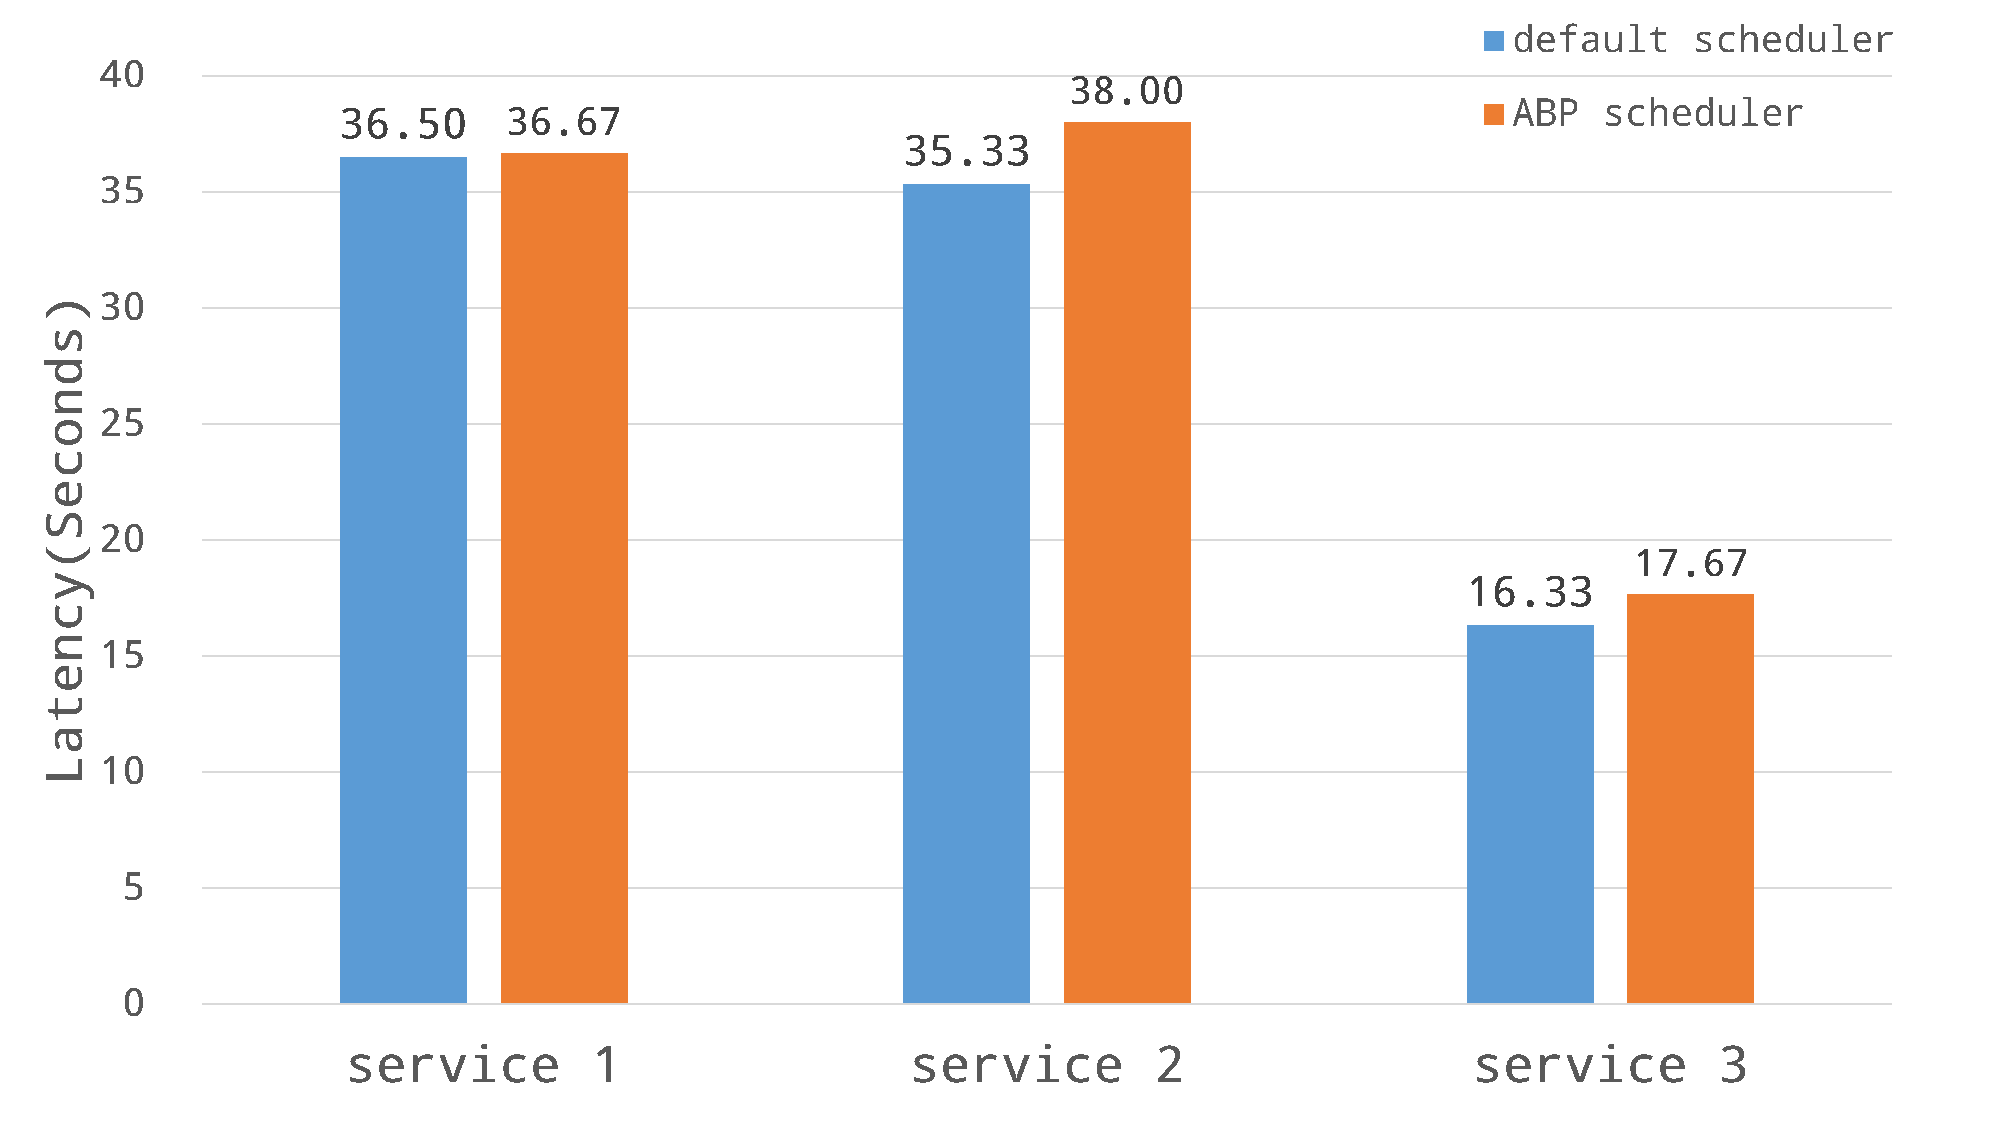
\includegraphics[width=0.9\textwidth]{./figure/baseline}
\bicaption[fig:baseline]{创建服务耗时基准}{\textbf{服务创建耗时}: 以每个服务的副本数要求为2且有2个任务实例作为本次实验的基准}{Fig}{\textbf{Services Creation}: creating each service with 2 tasks and 2 replicas, as the baseline of our experiments}
\end{figure}

我们将测试场景\ref{create1}中的测试结果作为衡量不同系统在容器云集群中创建启动相应服务所需耗时的基准值。从图\ref{fig:baseline}中可以看出,相关服务在本课题的系统中启动耗时相比默认的Docker \emph{swarm}框架要略微高一些。这是由于相比Docker \emph{swarm},本课题提出的系统需要额外从Docker \emph{registry}(并非本地的Docker \emph{registry}镜像服务)获取Docker镜像文件的元数据造成的耗时。但由于镜像元数据的数据量很小,因此这个额外耗时主要消耗在建立网络连接过程,根据实验过程中的多次测试验证,整个过程耗时很少超过3秒。对比下载整个镜像文件的耗时造成的延迟损失,我们认为这部分的延迟开销是可以接受的。除此之外,通过对实验观测到的数据进行分析,我们发现本系统的标准差比Docker \emph{swarm}框架中的标准差高出1秒左右,这主要是由于从国内实验环境连接到位于美国的Docker \emph{registry}服务的网络环境不稳定导致的。

\begin{figure}[htbp]
\centering
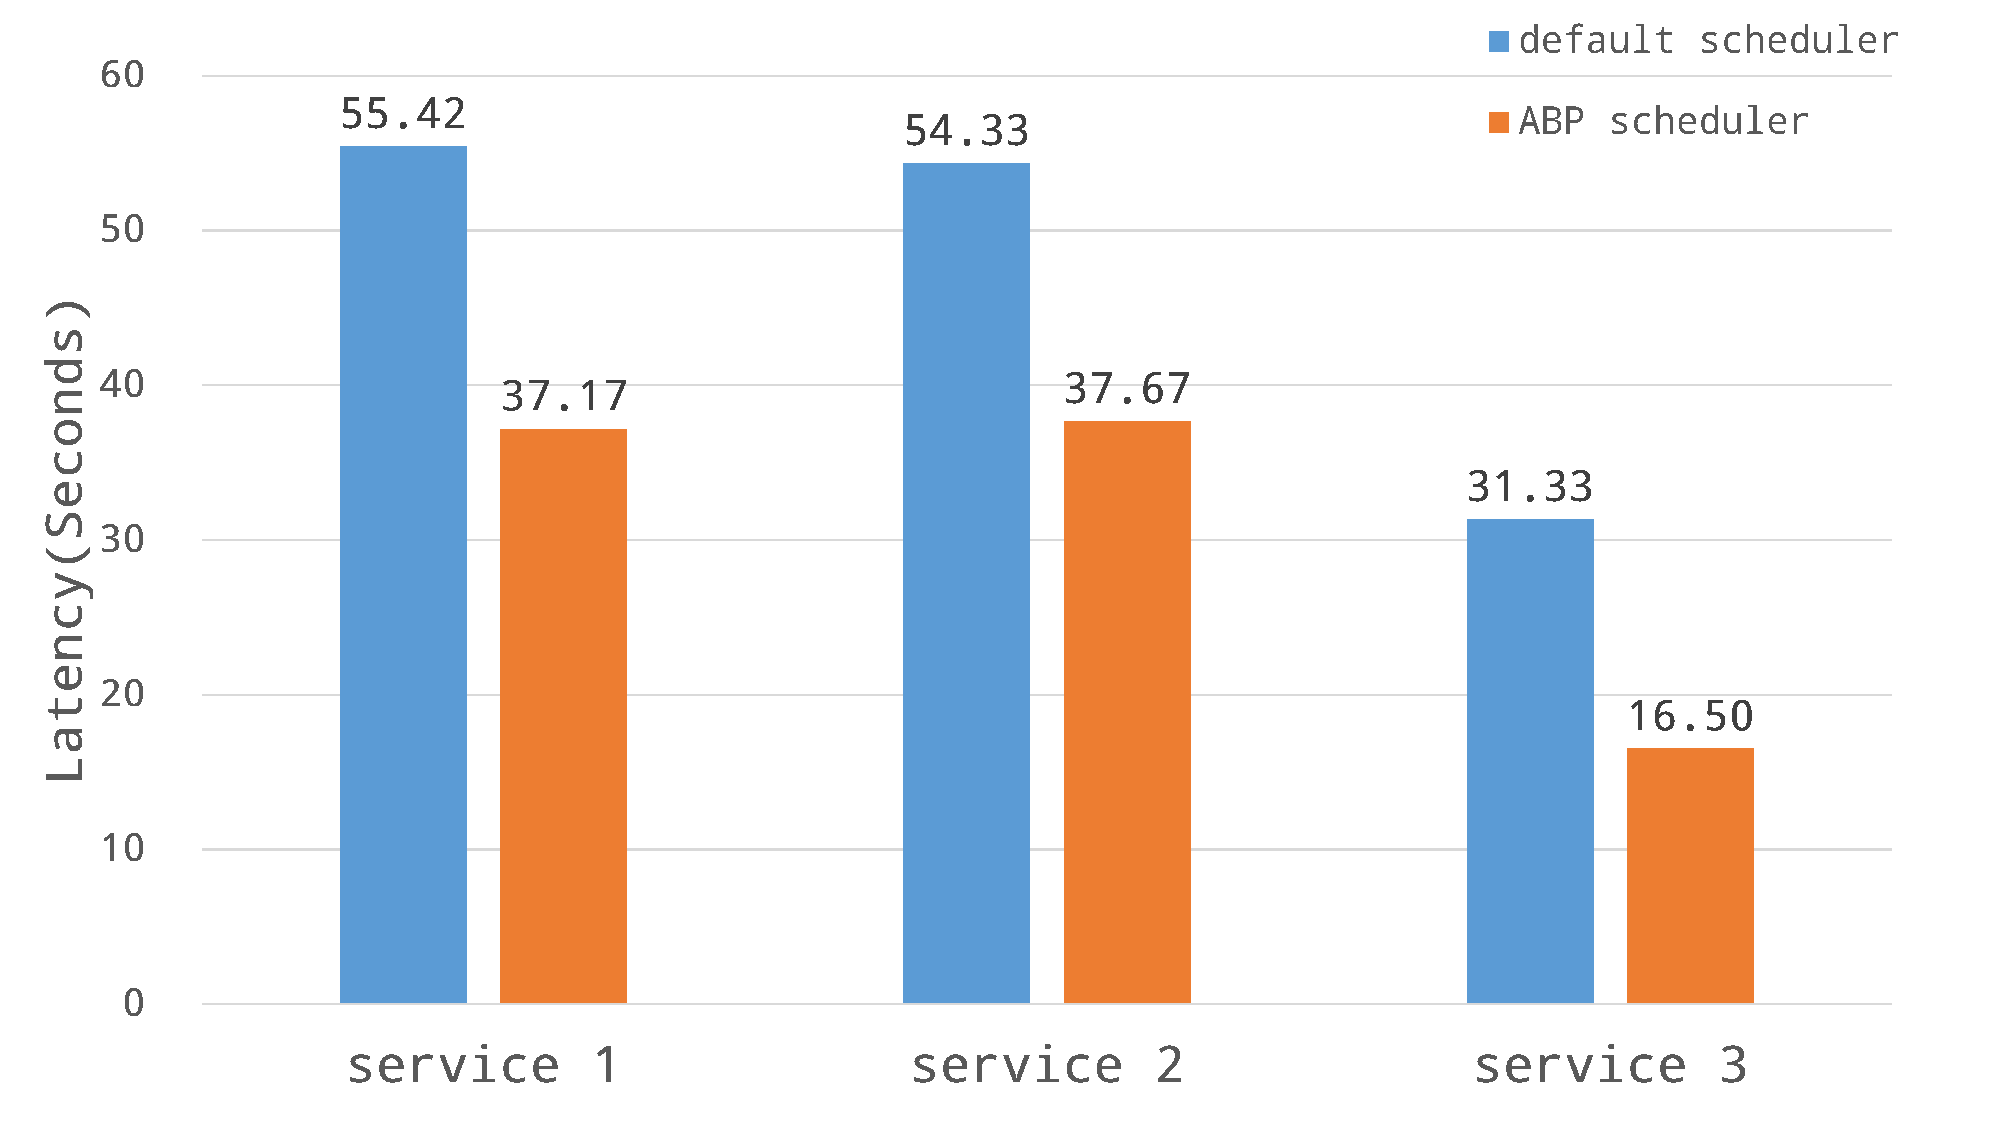
\includegraphics[width=0.9\textwidth]{./figure/4ins2rep}
\bicaption[fig:4ins]{创建服务:每个服务副本数要求为2且有4个任务实例}{\textbf{服务创建耗时}:每个服务副本数要求为2且有4个任务实例}{Fig}{\textbf{Services Creation}: creating each service with 4 tasks and 2 replicas}
\end{figure}

从图\ref{fig:4ins}中可知,在测试场景\ref{create2}下,服务在容器云中通过本课题提出的系统比通过Docker \emph{swarm}框架能以更快的速度完成创建和启动。对比图\ref{fig:4ins}和图\ref{fig:baseline},我们可以发现随着任务实例数的增加,Docker \emph{swarm}框架需要接近两倍于基准的延迟等待时间来完成相应服务的创建启动过程。Docker \emph{swarm}框架中服务启动出现大幅度延迟的原因是容器集群和本地Docker \emph{registry}镜像服务间的网络带宽。根据在之前的实验环境\ref{req:registry_mirror},容器集群和本地Docker \emph{registry}镜像服务间的网络带宽为100Mbps。在测试场景\ref{create2}下,每个服务在容器云中有4个任务实例需要创建并运行。在Docker \emph{swarm}框架下,每个服务的4个任务实例被平均分配到集群的4个节点上,集群内的网络请求数目随着实例数目增长而增长(最多可达到集群内的节点数目)。当这4个节点接受了对应的任务实例后,节点上的Docker Engine会开始从本地Docker \emph{registry}镜像服务获取相应的Docker镜像。在测试场景\ref{create1}下,由于每个服务只有2个任务实例,所以每次服务创建时只有两个镜像下载请求来平分容器集群和本地Docker \emph{registry}镜像服务间的网络带宽。在测试场景\ref{create2}中,因为有4个镜像下载请求同时存在,导致网络带宽由原来被2个下载请求平分变成被4个下载请求平分。网络请求数目增加了一倍,使得每个下载请求的传输速度只有测试场景\ref{create1}中的一半,导致整体下载耗时增加了一倍。与Docker \emph{swarm}框架相反,在本课题提出的系统中,为了满足服务自身的可用性目标,每个服务的4个任务实例被分配到了集群内的2个节点上。这使得系统在满足服务可用性要求的前提下,整个容器集群中只有两个节点发出下载请求使用网络。容器集群和本地Docker \emph{registry}镜像服务间的100Mbps网络带宽在实验场景\ref{create1}中和实验场景\ref{create2}中都是同时被两个下载请求平分,并没有增加集群内的网络流量。每个下载请求的传输速度没有变化,因此服务整体的启动延迟在实验场景\ref{create2}中和实验场景\ref{create1}中几乎一致。

\begin{figure}[htbp]
\centering
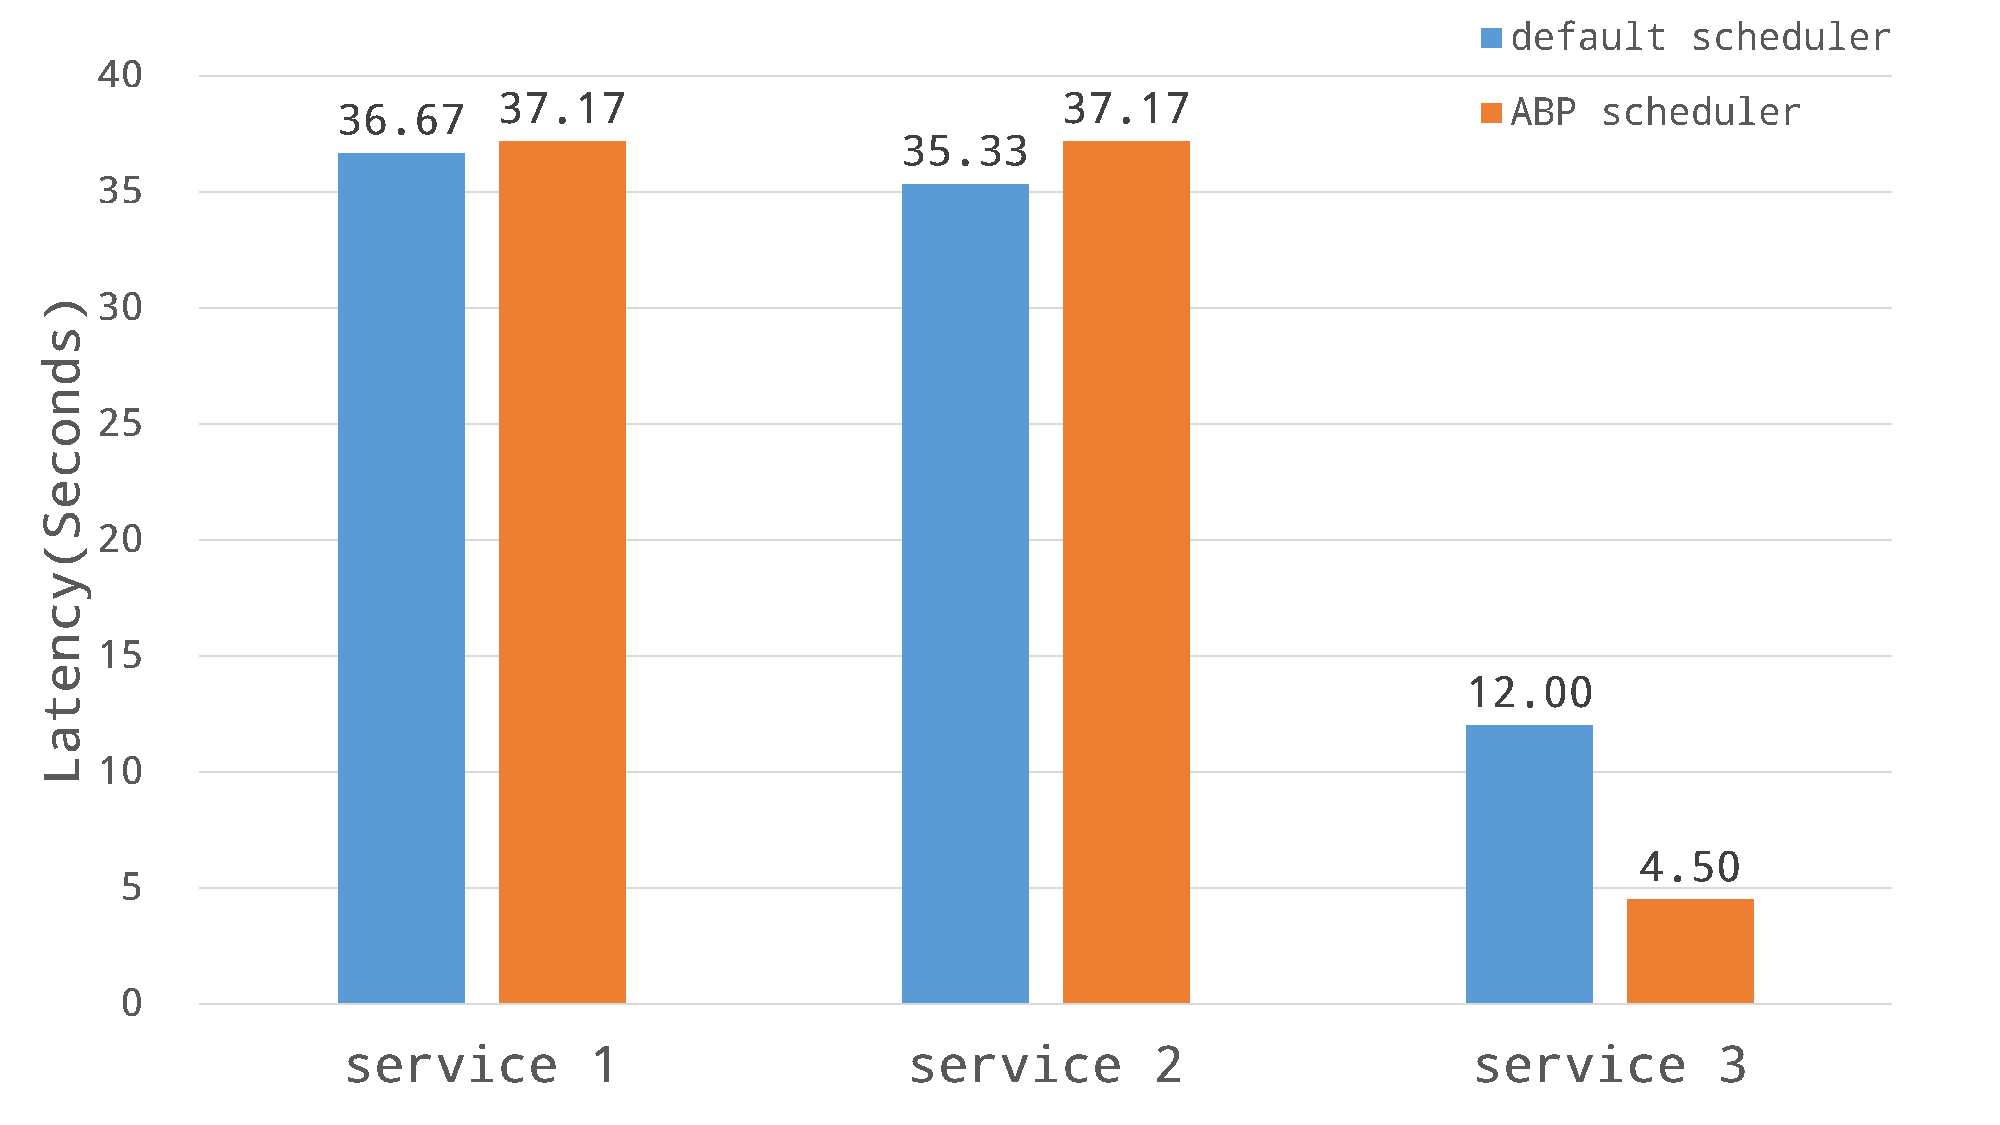
\includegraphics[width=0.9\textwidth]{./figure/132}
\bicaption[fig:132]{按照\emph{service1},\emph{service3}和\emph{service2}的顺序依次创建服务:每个服务副本数要求为2且有2个任务实例}{\textbf{服务创建耗时}: 每个服务副本数要求为2且有2个任务实例,按照\emph{service1},\emph{service3}和\emph{service2}的顺序依次创建各个服务}{Fig}{\textbf{Services Creation}: creating services with 2 tasks and 2 replicas in a sequence of \emph{service1}, \emph{service3} and \emph{service2}}
\end{figure}

服务用于满足自身可用性要求的副本数常常并不等于满足自身负载需求的实例数。在实际中,相比满足可用性目标的副本个数,服务往往需要更多的实例来应对自身的负载需要来保证服务本身的质量。为了评估本课题提出的系统在该场景下的表现,我们设计了实验场景\ref{create3}并进行了相关实验,实验结果如图\ref{fig:132}所示。从图\ref{fig:132}中可以明显看出,对比Docker \emph{swarm}框架,\emph{service3}整体的启动延迟时间在本课题提出的系统中显著降低。这主要是如我们在第\ref{chap:sys_design}章中所说,因为本课题提出的系统在资源分配阶段考虑了Docker镜像中的层级文件和容器集群节点上保存的Docker镜像文件缓存相关性,在同一节点上的不同服务间共享了部分Docker镜像分层文件缓存,降低了服务在创建和启动方面的延迟。根据我们在前面准备部分\ref{req:serv_image}中相关Docker镜像的具体构成,服务\emph{service1}和服务\emph{service3}使用的应用镜像\emph{image1}和\emph{image3}都包含了来自\emph{debian:jessie}这个基础镜像的同样的层级文件。在服务\emph{service1}被创建的过程中,\emph{debian:jessie}镜像的层级文件会被这些准备运行服务\emph{service1}相关任务实例的集群节点下载并缓存。在对服务\emph{service3}的任务实例基于负载应对选择托管的容器集群节点时,根据在\ref{sec:sec:node_selection}节中的设计,本课题提出的系统将优先把相应任务实例分布到那些已经运行了服务\emph{service1}任务实例的集群节点。在实验过程中,我们也发现如果按照\emph{service1}、\emph{service2}和\emph{service3}的顺序创建相关服务,服务\emph{service3}的任务实例在Docker \emph{swarm}框架下有时也会被分发到运行着服务\emph{service1}任务实例的集群节点上。这主要是当集群中节点运行的任务实例数目相同时,Docker \emph{swarm}框架根据节点的通用唯一识别码(Universally Unique Identifier,UUID)按照字典序进行任务的分发和调度,集群中节点的UUID则由节点上的Docker Engine在启动的时候基于sha256算法随机生成。

\subsection{服务伸缩实验}\label{sec:serv_scale}
我们已经在第\ref{sec:serv_creation}节中显示了本课题提出的系统在服务创建和启动方面相比Docker \emph{swarm}框架带来的显著提升。虽然服务创建的表现对保障服务质量很重要,但是在动态变化的负载压力下,服务进行伸缩的性能表现则是关键。当负载增长时,服务需要进行扩展(scale-out)以保证服务质量;当负载降低时,服务需要进行收缩(scale-in)从而减少不必要的资源,提高资源使用率,降低成本。降低服务伸缩过程任务实例的启动/关闭延迟可以增强服务整体应对负载的灵活性,从而更好地保证服务的质量。为了验证本课题提出的系统在服务扩展和服务收缩场景下对任务实例启动延迟的影响,我们设计了如下两个实验并和Docker \emph{swarm}框架进行了对比:

\begin{enumerate}
\item\label{scale1} 基于服务创建实验\ref{create1}中的要求创建服务,然后将相应的服务扩展到4个任务实例,最后再将相应服务收缩到2个任务实例。对服务\emph{service1},\emph{service2}和\emph{service3}独立进行上述实验,每次实验之前重置整个实验环境,保证不同服务的实验之间没有影响。
\item\label{scale2} 基于服务创建实验\ref{create3}创建服务,分别用Docker \emph{swarm}和本文提出的系统按照\emph{service1},\emph{service3}和\emph{service2}的顺序依次创建服务。每个服务有2个任务实例,同时为了满足\ref{req:serv_aval}中提到的可用性要求,在本课题提出的系统中为每个服务设置2个副本。随后,将服务\emph{service1}扩展到4个任务实例。
\end{enumerate}

以上两个实验设计均包含了服务的扩展和伸缩部分,但是这两个设计针对的场景侧重点不同。实验设计场景\ref{scale1}主要通过对各个服务的伸缩性能进行独立实验来验证本系统在单一服务场景下对单个服务伸缩性能的影响;验设计场景\ref{scale2}通过从所有服务中选择一个服务来进行伸缩实验从而来验证本系统在多服务的场景下对其中一个服务进行伸缩时的性能影响。以下将根据以上两个设计场景下的实验结果整合后,分为服务扩展和服务收缩两部分进行介绍和说明。

\subsubsection{服务扩展表现}\label{sec:scaleout}

\begin{figure}[htbp]
\centering
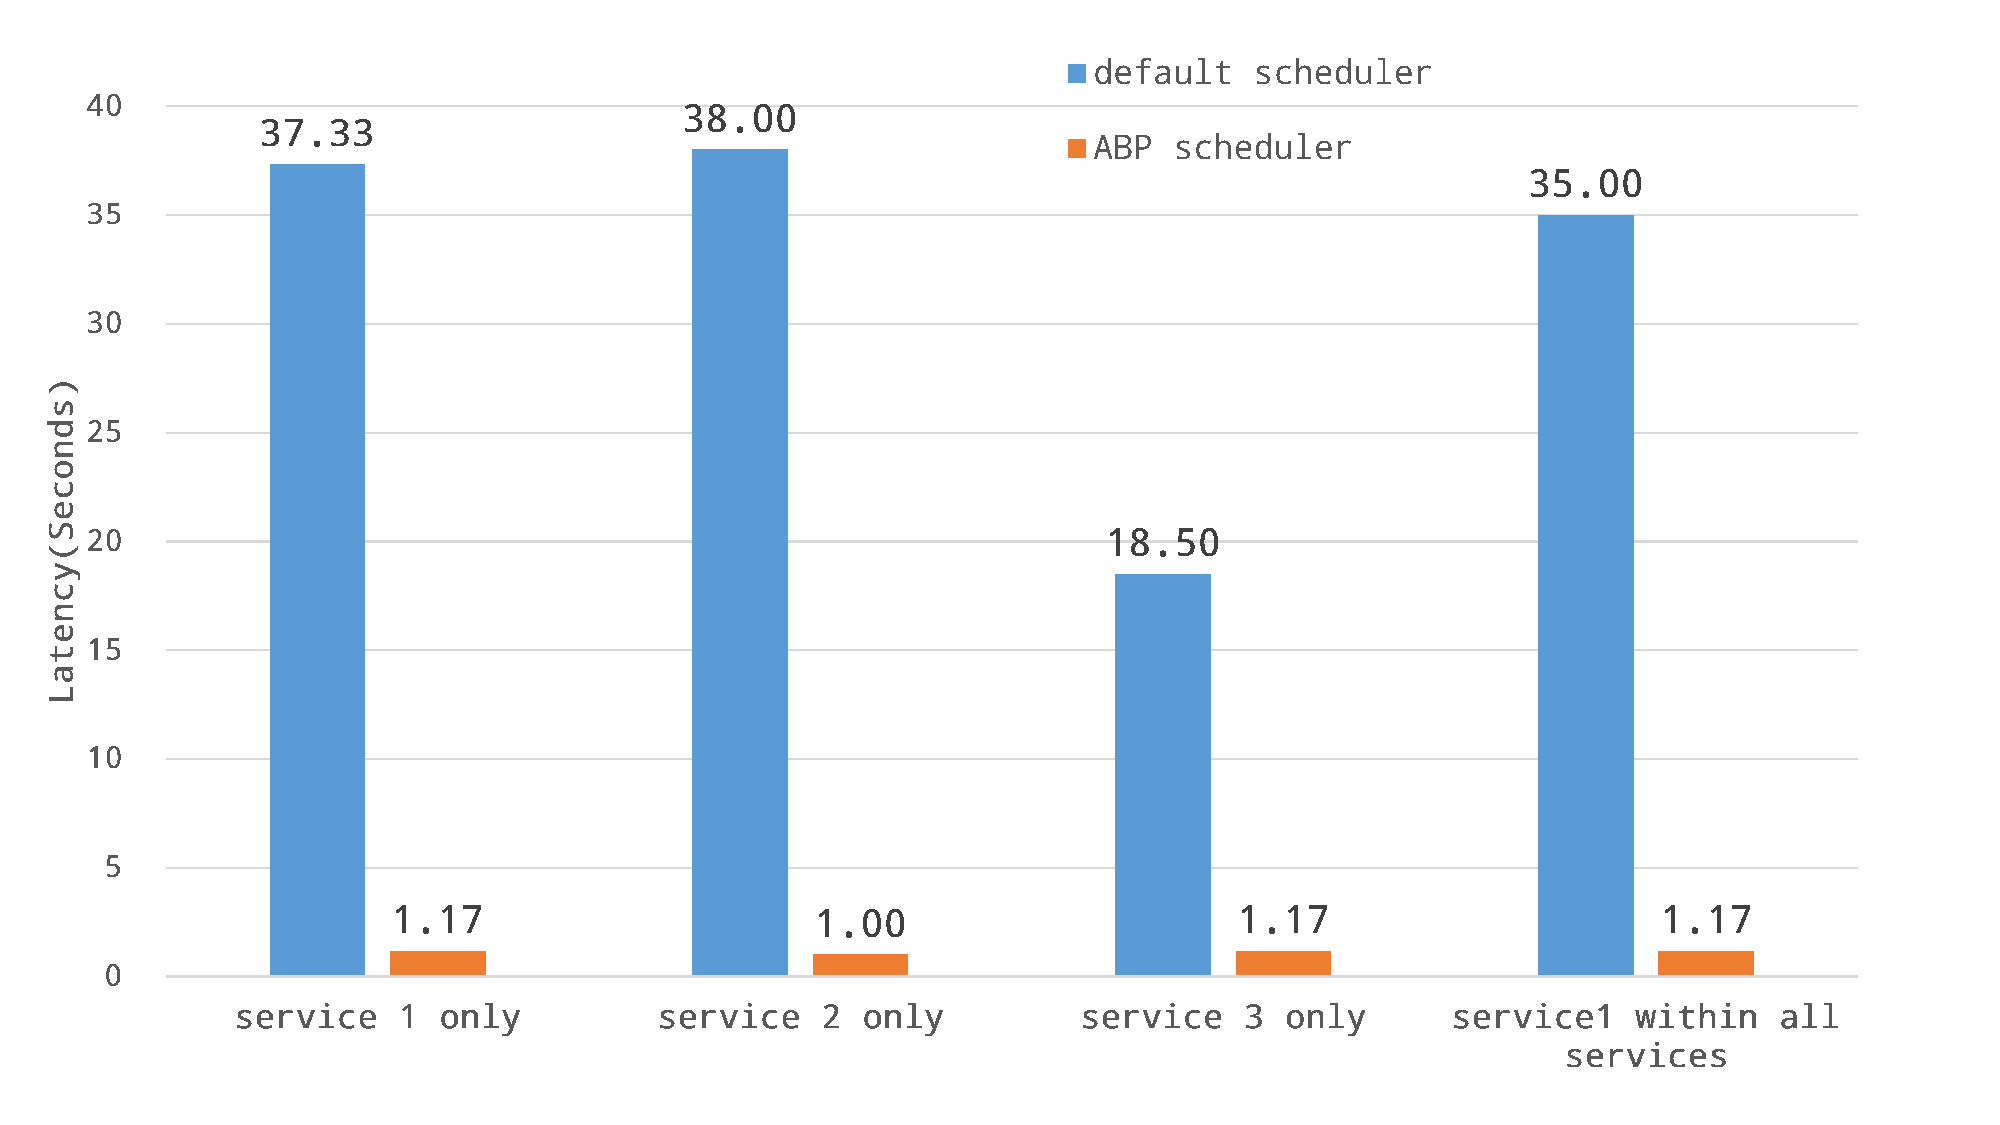
\includegraphics[width=0.9\textwidth]{./figure/scaleout}
\bicaption[fig:scaleout]{服务扩展}{\textbf{服务扩展-应对负载增加}}{Fig}{Service Scaling Out}
\end{figure}

图\ref{fig:scaleout}展示了服务扩展操作在本课题提出的系统中有一个显著的加速,服务整体的扩展延迟比在Docker \emph{swarm}框架中有大幅度降低。通过本课题提出的系统,容器集群中的服务能在极短的延迟(基本不超过2s)下完成伸缩,这显然在负载急剧增长的场景下能对提升服务整体的服务质量有极大的帮助。与之相对,我们发现在Docker \emph{swarm}框架下,每个服务的扩展延迟几乎等于他们创建阶段的耗时,而创建耗时又和服务所使用的Docker镜像大小密切相关。鉴于Docker \emph{swarm}框架中服务的任务实例常常被尽可能平均地分发到了整个容器集群中所有满足限制条件的节点上,使得整个容器集群中的节点上任务实例近似一致。而在整个容器集群中,并不是所有节点都拥有相应服务所依赖的层级文件缓存。这就导致有些任务实例被分发到了一个完全没有任何相关依赖层级文件缓存的集群节点上,而这些节点则需要下载对应服务所需要的完整Docker镜像从而来运行这些任务实例。当服务在本课题提出的系统中需要进行扩展的时候,系统会根据节点上的层级文件缓存和当前服务所需Docker镜像中层级文件的重合度以及节点的资源利用率来从容器集群中选择合适的节点来运行扩展的任务实例。因此在系统中被选择用作运行新任务实例的节点不需要下载全部的Docker镜像文件,加快了扩展任务实例的启动时间,从而降低了服务扩展操作的整体延时。

针对伸缩实验场景\ref{scale2},我们从图\ref{fig:scaleout}中还可以发现:按照\emph{service1},\emph{service3}和\emph{service2}的顺序创建相应服务后,在Docker \emph{swarm}框架下对服务\emph{service1}进行扩展的时候服务扩展所需要的耗时相比单独对服务\emph{service1}进行扩展时所要的耗时降低了一点。造成这个现象的原因是在该场景下容器集群中所有节点都有了底层基础镜像\emph{debian:jessie}镜像的层级文件缓存从而减少了这部分文件下载所需要的耗时。在该场景下,由于集群只有4个节点并且服务按照\emph{service1}、\emph{service3}和\emph{service2}的顺序依次创建,服务\emph{service1}扩展产生的任务实例被分发到集群中尚未运行服务\emph{service1}任务实例的两个节点。我们在之前准备环境\ref{req:serv_image}部分中已经说明了服务\emph{service1}和服务\emph{service3}使用的应用镜像\emph{image1}和\emph{image3}由于都使用\emph{debian:jessie}镜像作为基础镜像,因此这两个应用镜像共享这部分的层级文件。因此在对服务\emph{service1}进行扩展的时候,这两个节点上已经运行了服务\emph{service3}的相关任务实例,因此针对\emph{debian:jessie}镜像这一部分的层级文件可以直接利用存储在各自节点上的缓存而不需要再次下载。不过我们从图\ref{fig:scaleout}中也可以发现,即使利用了这部分缓存的共享层级文件,对服务扩展操作的加速仍然只是杯水车薪。在Docker \emph{swarm}框架中,运行扩展任务实例的节点仍然需要下载约270MB大小的层级文件以安装应用运行所需要的\emph{Golang}运行时环境。与之相对,在本课题提出的系统中,运行扩展任务实例的节点由于在本地已经缓存了服务\emph{service1}使用的Docker容器镜像,因此避免了对相应层级文件的下载耗时和网络开销。

\subsubsection{服务收缩表现}\label{sec:scalein}

当服务在Docker \emph{swarm}框架中进行收缩时,Docker \emph{swarm}框架会从所有节点中根据运行该服务相应任务实例数目进行选择并试图将集群中节点上运行的实例数目接近一致。在相同场景下,如我们在之前的设计章节%\ref{algo:scalein}
中所说,本课题提出的系统则根据任务实例的优势资源相对节点总资源的占比进行选择。

\begin{figure}[htbp]
\centering
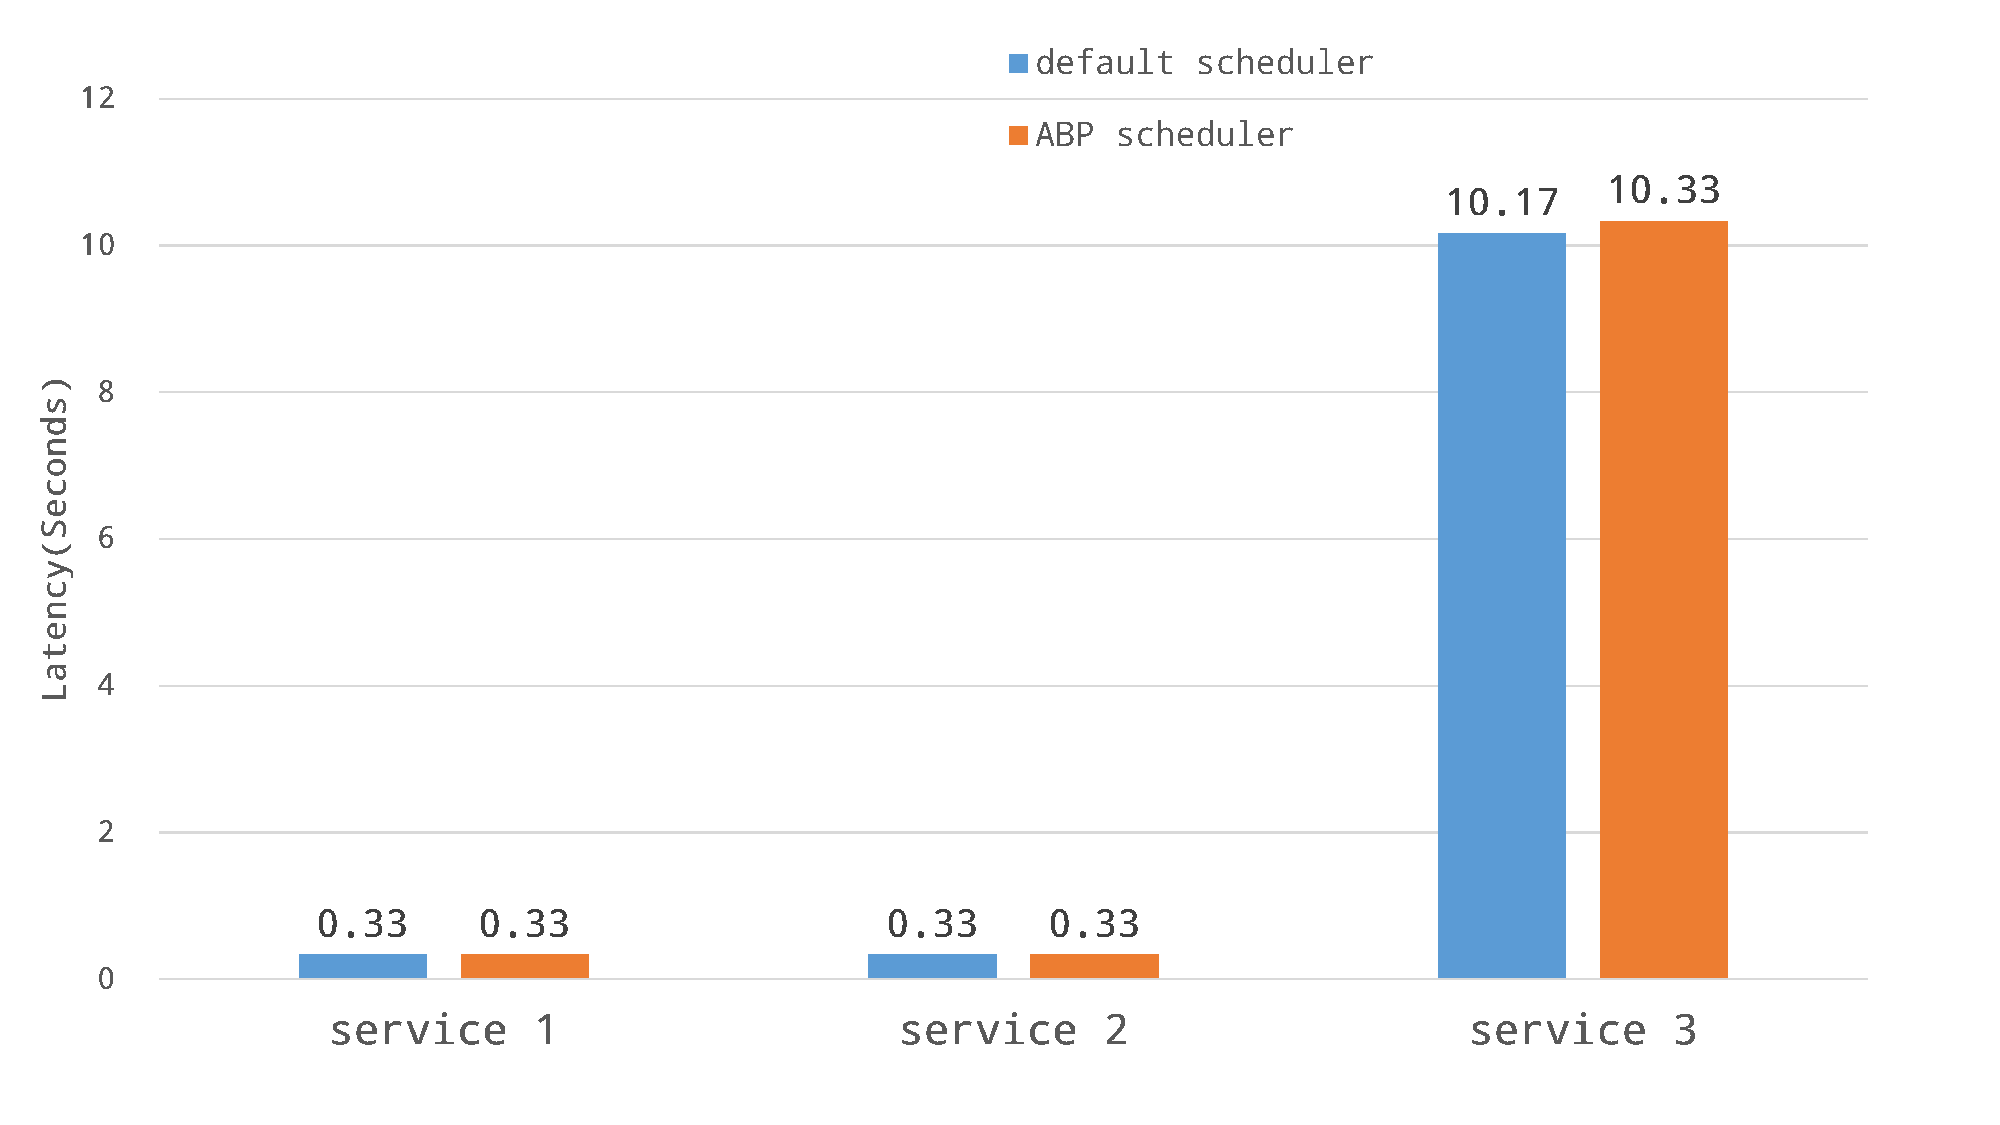
\includegraphics[width=0.9\textwidth]{./figure/scalein}
\bicaption[fig:scalein]{服务收缩}{\textbf{服务收缩-应对负载降低}}{Fig}{Service Scaling In}
\end{figure}

图\ref{fig:scalein}显示了服务收缩在Docker \emph{swarm}框架和本课题提出的系统中所需要的延迟时间。我们由图\ref{fig:scalein}可以发现服务在Docker \emph{swarm}框架和本课题提出的系统中几乎都是立即完成了相应的服务收缩操作,收缩操作的时间延迟基本不超过0.5秒。服务\emph{service3}的收缩操作延迟相比其他两个服务显得很异常,但是也这是在预期之中的。这主要是因为服务\emph{service3}运行的是一段包含了无限循环的shell脚本,导致运行相应任务实例的容器无法响应该节点上的Docker Engine正常发送的停止请求。根据Docker Engine中定义的容器关闭规则,在经过一个既定的等待期(默认10秒)之后,Docker Engine将通过发送SIGKILL的方式强制杀死运行对应任务实例的容器进程。通过对比,我们可以发现服务在Docker \emph{swarm}框架和本课题提出的系统中进行收缩需要的延迟几乎毫无差别。

\section{本章小结}


